\section{Experiments}
\label{sec:Experiments}

\begin{table*}[!t]    %[htbp]
\tablestyle{5pt}{1.0}

\newcommand{\downtiny}[1]{{\!\tiny{#1}}}

\setlength\tabcolsep{5pt}
% \def\w{20pt} 
\scalebox{1}{
    \begin{tabular}{lcccccccc}
    \multirow{2}{*}{\textbf{Methods}} & \multirow{2}{*}{\textbf{MVBench}} & \multirow{2}{*}{\textbf{LongVideoBench}} & \multirow{2}{*}{\textbf{MLVU}} & \multicolumn{4}{c}{\textbf{VideoMME}} & \multirow{2}{*}{\textbf{Average (\%)}} \\
        &  &  &  & \textbf{Overall} & \textbf{Short} & \textbf{Medium} & \textbf{Long} &  \\
    \shline
    \multicolumn{9}{l}{\textit{Upper Bound}} \\
    \textcolor[rgb]{ .502,  .502,  .502}{LLaVA-OV-7B} & \textcolor[rgb]{ .502,  .502,  .502}{56.9} & \textcolor[rgb]{ .502,  .502,  .502}{56.4} & \textcolor[rgb]{ .502,  .502,  .502}{63.0} & \textcolor[rgb]{ .502,  .502,  .502}{58.6} & 
    \textcolor[rgb]{ .502,  .502,  .502}{70.3} &
    \textcolor[rgb]{ .502,  .502,  .502}{56.6} &
    \textcolor[rgb]{ .502,  .502,  .502}{48.8} &
    \textcolor[rgb]{ .502,  .502,  .502}{100.0} \\
    \hline
    \multicolumn{9}{l}{\textit{Retention Ratio=30\%}} \\
    DyCoke \downtiny{[CVPR'25]} & 56.6 & 54.7 & 60.3 & 56.1 & 67.1 & 54.6 & 46.6 & 96.5 \\
    \hline
    \multicolumn{9}{l}{\textit{Retention Ratio=25\%}} \\
    Random & 54.2 & 52.7 & 59.7 & 55.6 & 65.4 & 53.0 & 48.3 & 94.8 \\
    \hline
    FastV \downtiny{[ECCV'24]} & 55.5 & 53.3 & 59.6 & 55.3 & 65.0 & 53.8 & 47.0 & 94.9 \\
    PDrop \downtiny{[CVPR'25]} & 55.3 & 51.3 & 57.1 & 55.5 & 64.7 & 53.1 & 48.7 & 94.1 \\
    SparseVLM \downtiny{[ICML'25]} & 56.4 & 53.9 & 60.7 & 57.3 & 68.4 & 55.2  & 48.1 & 97.5 \\
    DyCoke \downtiny{[CVPR'25]} & 49.5 & 48.1 & 55.8 & 51.0 & 61.1 & 48.6 & 43.2 & 87.0 \\
    \rowcolor[rgb]{ .949,  .949,  .949}
    \textbf{VidCom$^2$} & \textbf{57.2} & \textbf{54.9} & \textbf{62.5} & \textbf{58.6} & \textbf{69.8} & \textbf{56.4} & \textbf{49.4} & \textbf{99.6} \\
    \hline
    \multicolumn{9}{l}{\textit{Retention Ratio=15\%}} \\
    FastV \downtiny{[ECCV'24]} & 51.6 & 48.3 & 55.0 & 48.1 & 51.4 & 49.4 & 43.3 & 85.0 \\
    PDrop \downtiny{[CVPR'25]} & 53.2 & 47.6 & 54.7 & 50.1 & 58.7 & 48.7 & 45.0 & 87.4 \\
    SparseVLM \downtiny{[ICML'25]} & 52.9 & 49.7 & 57.4 & 53.4 & 61.0 & 52.1 & 47.0 & 91.2 \\
    \rowcolor[rgb]{ .949,  .949,  .949}
    \textbf{VidCom$^2$} & \textbf{54.3} & \textbf{52.0} & \textbf{58.9} & \textbf{56.2} & \textbf{65.8} & \textbf{54.8} & \textbf{48.1} & \textbf{95.1} \\
    \shline
    \multicolumn{9}{l}{\textit{Upper Bound}} \\
    \textcolor[rgb]{ .502,  .502,  .502}{LLaVA-Video-7B} & \textcolor[rgb]{ .502,  .502,  .502}{60.4} & \textcolor[rgb]{ .502,  .502,  .502}{59.6} & \textcolor[rgb]{ .502,  .502,  .502}{70.3} & \textcolor[rgb]{ .502,  .502,  .502}{64.3} & 
    \textcolor[rgb]{ .502,  .502,  .502}{77.2} &
    \textcolor[rgb]{ .502,  .502,  .502}{62.1} & 
    \textcolor[rgb]{ .502,  .502,  .502}{53.4} & \textcolor[rgb]{ .502,  .502,  .502}{100.0} \\
    \hline
    \multicolumn{9}{l}
    {\textit{Retention Ratio=30\%}} \\
    DyCoke \downtiny{[CVPR'25]} & 57.5 & 55.5 & 60.6 & 61.3 & 73.4 & 59.3 & 51.2 & 93.8 \\
    \hline
    {\textit{Retention Ratio=25\%}} \\
    FastV \downtiny{[ECCV'24]} & 53.8 & 51.2 & 57.8 & 59.3 & 67.1 & 60.0 & \textbf{50.8} & 89.7 \\
    SparseVLM \downtiny{[ICML'25]} & 55.4 & 54.2 & 58.9 & 60.1 & 71.1 & 59.1 & 50.1 & 91.6 \\
    DyCoke \downtiny{[CVPR'25]} & 50.8 & 53.0 & 56.9 & 56.1 & 65.8 & 53.6 & 48.9 & 86.3 \\
    \rowcolor[rgb]{ .949,  .949,  .949}
    \textbf{VidCom$^2$} & \textbf{57.0} & \textbf{55.5} & \textbf{59.0} & \textbf{61.7} & \textbf{73.0} & \textbf{61.7} & 50.0 & \textbf{93.6} \\
    \hline
    \multicolumn{9}{l}{\textit{Retention Ratio=15\%}} \\
    FastV \downtiny{[ECCV'24]} & 44.0 & 44.6 & 53.8 & 51.3 & 56.4 & 51.1 & 46.2 & 78.0 \\
    % PDrop \downtiny{[CVPR'25]} & 49.9 & 48.8 &   & 54.8 & 62.8 & 52.2 & 47.4 &  \\
    SparseVLM \downtiny{[ICML'25]} & 53.1 & \textbf{52.7} & 56.2 & 55.7 & 65.0 & 53.9 & 48.3 & 86.3 \\
    \rowcolor[rgb]{ .949,  .949,  .949}
    \textbf{VidCom$^2$} & \textbf{53.3} & 51.5 & \textbf{56.8} & \textbf{58.3} & \textbf{68.0} & \textbf{57.3} & \textbf{49.7} & \textbf{88.5} \\
    
    \end{tabular}%    
    }
    \vspace{-2mm}
    \caption{\textbf{Performance comparison with other baselines with LLaVA-OV-7B and LLaVA-Video-7B across different benchmarks.} ``Average'' shows the mean performance across different benchmarks. 
    DyCoke requires pruning similar tokens from consecutive 4 frames, making it not possible for the retention ratio of $R<25\%$.
    }
    \vspace{-5mm}
  \label{tab:main_results}%
\end{table*}%


\subsection{Experimental Setting}
\label{subsec:Setting}


\noindent \textbf{Benchmark.} We conduct comprehensive comparative experiments across multiple benchmarks, including: MVBench~\cite{li2024mvbench}, LongVideoBench~\cite{wu2024longvideobench}, MLVU~\cite{zhou2024mlvu}, VideoMME~\cite{fu2024videomme}, EgoSchema~\cite{mangalam2023egoschema}, and PerceptionTest~\cite{patraucean2023perception}, employing LMMs-Eval~\cite{zhang2024lmms} evaluation framework. More details are in Appendix~\ref{sec:appendix/benchmarks}.


\noindent \textbf{Implementations.} We evaluate our method on popular VideoLLMs: LLaVA-OneVision (LLaVA-OV)~\cite{li2024llava-ov}, LLaVA-Video~\cite{zhang2024llava-video}, and Qwen2-VL~\cite{Wang:Qwen2-VL}. Detailed model information is in Appendix~\ref{sec:appendix/models}. All experiments use NVIDIA A100-SXM4-80GB GPUs.


\noindent \textbf{Baselines.} We evaluate our method against various training-free token compression strategies, including: FastV~\cite{Chen:FastV}, PDrop~\cite{xing2024pdrop}, SparseVLM~\cite{Zhang:SparseVLM}, and DyCoke~\cite{tao2024dycoke}, more introduction can be seen in Appendix~\ref{sec:appendix/baselines}. Following SparseVLM, we use the ``equivalent retention ratio''\footnote{``Equivalent retention ratio'' represents the average percentage of visual tokens retained across all LLM layers.} for fair comparisons. Unlike others, DyCoke compresses both visual tokens and KV cache. For fair comparison, we evaluate only on its token compression strategy.

\begin{figure}[t]
    \centering
    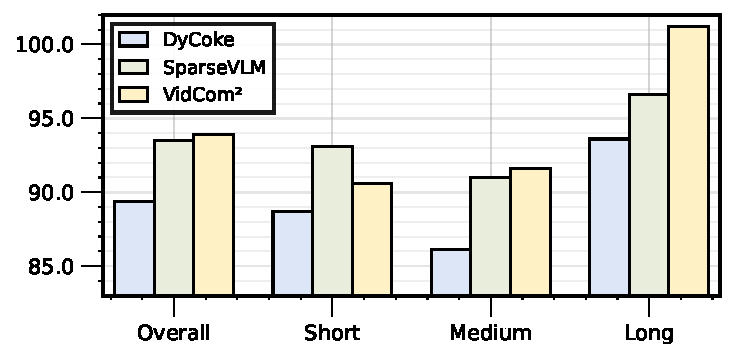
\includegraphics[width=\linewidth]{latex/figures/comparison_qwen2_vl.pdf}
    \vspace{-7mm}
    \caption{\textbf{Performance with Qwen2-VL.} At $R=25\%$, VidCom$^2$ surpasses DyCoke and SparseVLM by \textbf{7.6\%} and \textbf{4.6\%} of original performance in long video tasks.} 
    \vspace{-5mm}
    \label{fig:qwen_2_vl}
\end{figure}

\subsection{Main Comparisons}
\label{subsec:Comparison}

% \noindent \textbf{Performance Comparisons.}
\paragraph{Performance Comparisons.} 

Table~\ref{tab:main_results} presents a comparative analysis of our VidCom$^2$ against multiple token compression methods across various benchmarks. The experimental results reveal \textbf{\emph{two key performance advantages}} of VidCom$^2$:


\begin{table}[!t]
\tablestyle{5pt}{1.0}
\newcommand{\downtiny}[1]{{\!\tiny{#1}}}
\setlength\tabcolsep{8.8pt}
\scalebox{1}{
    \begin{tabular}{lcc}
    \textbf{Methods} & \textbf{EgoSchema} & \textbf{PerceptionTest} \\
    \shline
    \multicolumn{3}{l}{\textit{Upper Bound}} \\
    \textcolor[rgb]{.502,.502,.502}{LLaVA-OV-7B} & \textcolor[rgb]{.502,.502,.502}{60.4 (100\%)} & \textcolor[rgb]{.502,.502,.502}{57.1 (100\%)} \\
    \hline
    \multicolumn{3}{l}{\textit{Retention Ratio=25\%}} \\
    FastV \downtiny{[ECCV'24]} & 57.5 (95.2\%) & 55.4 (97.0\%) \\
    PDrop \downtiny{[CVPR'25]} & 58.0 (96.0\%) & 55.6 (97.4\%) \\
    DyCoke \downtiny{[CVPR'25]} & 59.5 (98.5\%) & 56.4 (98.8\%) \\
    \rowcolor[rgb]{.949,.949,.949}
    \textbf{VidCom$^2$} & \textbf{59.7 (98.8\%)} & \textbf{56.7 (99.3\%)} \\
    \end{tabular}
}
\vspace{-2mm}
\caption{\textbf{Performance comparison on EgoSchema and PerceptionTest.} Percentages represent ratios to the original performance of LLaVA-OV-7B.}
\vspace{-5mm}
\label{tab:more_comparisons}
\end{table}

\definecolor{greenrightcolor}{RGB}{0,144,81} 
\definecolor{redrightcolor}{RGB}{255,0,0} 
\definecolor{bluerightcolor}{RGB}{0,0,255} % 

\newcommand{\downtinya}[1]{{\!\textcolor{greenrightcolor}{\tiny{#1}}}}
\newcommand{\uptiny}[1]{{\!\textcolor{redrightcolor}{\tiny{#1}}}}
\newcommand{\downtinyb}[1]{{\!\textcolor{bluerightcolor}{\tiny{#1}}}}

\newcommand{\downtiny}[1]{{\!\tiny{#1}}}

\begin{table*}[!t]
\tablestyle{5pt}{1.0}
  \centering
  \setlength{\tabcolsep}{0.5pt} 
    \scalebox{1}{
    \begin{tabular}{lccccccc}
    \multirow{2}{*}{\textbf{Methods}} & \textbf{LLM Generation↓} & \textbf{Model Generation↓} & \textbf{Total↓}  & \textbf{GPU Peak↓} & \textbf{Throughput↑} & \multirow{2}{*}{\textbf{Performance↑}} \\
    & \textbf{Latency (s)} & \textbf{Latency (s)} & \textbf{Latency (min:sec)} & \textbf{Memory (GB)} & \textbf{(samples/s)} &  \\
    \shline
    \textcolor[rgb]{ .502,  .502,  .502}{LLaVA-OV-7B} & \textcolor[rgb]{ .502,  .502,  .502}{618.0} & \textcolor[rgb]{ .502,  .502,  .502}{1008.4} & 
    \textcolor[rgb]{ .502,  .502,  .502}{26:03} & 
    \textcolor[rgb]{ .502,  .502,  .502}{17.7} & 
    \textcolor[rgb]{ .502,  .502,  .502}{0.64} & \textcolor[rgb]{ .502,  .502,  .502}{56.9} \\
    
    \hline
    \multicolumn{7}{l}{\textit{Retention Ratio=25\%}} \\
    Random  & 178.2 \downtinya{(↓71.2\%)} & 566.0 \downtinya{(↓43.9\%)} & 18:44 \downtinya{(↓28.1\%)} & 16.0 \downtinya{(↓9.6\%)} & 0.89 \downtinya{(1.39$\times$)} & 54.6 \downtinya{(↓2.3)} \\

    \hline
    
    FastV \downtiny{[ECCV'24]}  & 260.9 \downtinya{(↓57.8\%)} & 648.6 \downtinya{(↓35.7\%)} & 20:07 \downtinya{(↓22.8\%)} & 24.7 \uptiny{(↑39.5\%)} & 0.83 \downtinya{(1.30$\times$)} &  55.5 \downtinya{(↓1.4)}  \\
    
    PDrop \downtiny{[CVPR'25]}  & 205.6 \downtinya{(↓66.7\%)} & 592.6 \downtinya{(↓41.2\%)} & 18:50 \downtinya{(↓27.7\%)} & 24.5 \uptiny{(↑38.4\%)} & 0.88 \downtinya{(1.38$\times$)} &  55.3 \downtinya{(↓1.6)}  \\
    
    SparseVLM \downtiny{[ICML'25]}  & 410.6 \downtinya{(↓33.6\%)} & 807.7 \downtinya{(↓19.9\%)} & 25:03 \downtinya{(↓3.8\%)} & 27.1 \uptiny{(↑53.1\%)} & 0.67 \downtinya{(1.05$\times$)} & 56.4 \downtinya{(↓0.5)} \\
    
    DyCoke \downtiny{[CVPR'25]}  & 205.2 \downtinya{(↓66.8\%)} & 598.0 \downtinya{(↓40.7\%)} & 18:56 \downtinya{(↓27.4\%)} & 16.1 \downtinya{(↓9.0\%)} & 0.88 \downtinya{(1.38$\times$)} & 49.5 \downtinya{(↓7.4)} \\
    
    \rowcolor[rgb]{ .949,  .949,  .949} \textbf{VidCom$^2$}  & \textbf{180.7 \downtinya{(↓70.8\%)}} & \textbf{574.7 \downtinya{(↓43.0\%)}} & \textbf{18:46 \downtinya{(↓28.0\%)}} & \textbf{16.0 \downtinya{(↓9.6\%)}} & \textbf{0.88 \downtinya{(1.38$\times$)}} & \textbf{57.2 \uptiny{(↑0.3)}} \\
    
    \hline
    \multicolumn{7}{l}{\textit{Retention Ratio=15\%}} \\
    Random  & 130.3 \downtinya{(↓78.9\%)} & 532.5 \downtinya{(↓47.2\%)} & 18:02 \downtinya{(↓30.8\%)} & 15.8 \downtinya{(↓10.7\%)} & 0.92 \downtinya{(1.44$\times$)} & 53.1 \downtinya{(↓3.8)} \\

    \hline
    
    FastV \downtiny{[ECCV'24]}  & 172.4 \downtinya{(↓72.1\%)} & 599.3 \downtinya{(↓40.6\%)} & 18:19 \downtinya{(↓29.7\%)} & 24.6 \uptiny{(↑39.0\%)} & 0.91 \downtinya{(1.42$\times$)} & 51.6 \downtinya{(↓5.3)} \\
    
    PDrop \downtiny{[CVPR'25]}  & 165.3 \downtinya{(↓73.3\%)} & 552.6 \downtinya{(↓45.2\%)} & 18:32 \downtinya{(↓28.9\%)} & 24.5 \uptiny{(↑38.4\%)} & 0.90 \downtinya{(1.41$\times$)} & 53.2 \downtinya{(↓3.7)} \\

    SparseVLM \downtiny{[ICML'25]}  & 370.4 \downtinya{(↓40.1\%)} & 764.8 \downtinya{(↓24.2\%)} & 24:09 \downtinya{(↓7.3\%)} & 27.1 \uptiny{(↑53.1\%)} & 0.69 \downtinya{(1.08$\times$)} & 52.9 \downtinya{(↓4.0)} \\
    
    \rowcolor[rgb]{ .949,  .949,  .949} \textbf{VidCom$^2$}  & \textbf{129.2 \downtinya{(↓79.1\%)}} & \textbf{533.0 \downtinya{(↓47.1\%)}} & \textbf{18:11 \downtinya{(↓30.2\%)}} & \textbf{15.8 \downtinya{(↓10.7\%)}} & \textbf{0.92 \downtinya{(1.44$\times$)}} & \textbf{54.3 \downtinya{(↓2.6)}} \\
    
    \end{tabular}%
    }
    \vspace{-2mm}
  \caption{\textbf{Efficiency comparisons on LLaVA-OV-7B.} ``LLM Generation Latency'': time for LLM-only response generation; ``Model Generation Latency'': time for model to generate response; ``Total Latency'': total time to complete MVBench; and  ``Throughput'': number of MVBench samples processed per second.}
  \label{tab:efficiency_comparisons}%
  \vspace{-5mm}
\end{table*}%



\noindent \textbf{(i) State-of-the-art Performance:} VidCom$^2$ demonstrates exceptional performance across diverse video understanding benchmarks. On LLaVA-OV and LLaVA-Video with compression ratio $R=25\%$, VidCom$^2$ substantially outperforms DyCoke by margins of \textbf{12.6\%} and \textbf{7.3\%}, respectively. Remarkably, VidCom$^2$ at $R=25\%$ (achieving 99.6\% performance retention) even surpasses DyCoke operating at a higher compression ratio of $R=30\%$ (96.5\% performance retention). This superiority extends to long-form video understanding tasks with Qwen2-VL (Figure~\ref{fig:qwen_2_vl}), where VidCom$^2$ achieves \textbf{101.2\%} performance on VideoMME (Long), surpassing both DyCoke (93.6\%) and SparseVLM (96.6\%) by substantial margins of \textbf{7.6\%} and \textbf{4.6\%}, respectively. Additional comparisons in Table~\ref{tab:more_comparisons} further validate the superior performance advantages of VidCom$^2$ across various video understanding scenarios.

\noindent \textbf{(ii) Robustness in Extreme Compression:} Under aggressive compression with $R=15\%$, most baselines such as FastV and PDrop exhibit significant performance degradation. Even the VideoLLM-specific method DyCoke \textbf{fails to achieve} such aggressive compression due to inherent design limitations.
However, VidCom$^2$ maintains robust performance, outperforming the second-best method SparseVLM by an average of \textbf{3.9\%} and \textbf{2.1\%} on LLaVA-OV and LLaVA-Video. 
This demonstrates VidCom$^2$'s superiority in frame-adaptive compression, dynamically adjusting intensity to preserve distinctive visual information.

Besides, we observe an interesting phenomenon that Intra-LLM methods (\textit{e.g.}, SparseVLM), which incorporate textual information, perform relatively better on long video tasks (\textit{e.g.}, LongVideoBench and VideoMME (long)) compared to shorter video benchmarks like MVBench and VideoMME (Short). For instance, SparseVLM slightly outperforms VidCom$^2$ on LongVideoBench with LLaVA-Video at $R=15\%$. This suggests that for longer videos with fixed frame counts, leveraging textual information for visual token compression helps VideoLLMs focus on text-relevant visual areas, potentially leading to improved performance.


% \noindent \textbf{Efficiency Comparisons.} 
\paragraph{Efficiency Comparisons.}

Beyond performance, Table~\ref{tab:efficiency_comparisons} presents comprehensive real-world inference efficiency comparisons among different token compression methods on MVBench, with all experiments conducted on four NVIDIA A100 GPUs. We follow the original implementation of each baseline method, and unless otherwise specified, Flash Attention 2~\cite{daoFlashAttention-2} is used as the efficient attention operator throughout comparisons. The comparison results in Table~\ref{tab:efficiency_comparisons} reveal \textbf{\emph{two key efficiency advantages}} of our VidCom$^2$:

\noindent \textbf{(i) State-of-the-art Efficiency:} VidCom$^2$ achieves remarkable inference efficiency, \textbf{comparable to} simple random token dropping. With 25\% visual tokens retained, the additional computation of VidCom$^2$ is \textbf{negligible} -- only 2.5s extra (\textbf{1.3\%} of LLM generation time) for the entire MVBench inference. Despite this minimal overhead, VidCom$^2$ significantly reduces both the LLM generation latency and overall model latency (primarily from ViT and LLM) by \textbf{70.8\%} and \textbf{43.0\%} respectively, achieving \textbf{1.38$\times$} throughput while maintaining \textbf{99.6\%} average performance across benchmarks. These results highlight the efficiency of VidCom$^2$ in accelerating inference for VideoLLMs.


\noindent \textbf{(ii) Efficient Operator Compatibility:} Pre-LLM methods like DyCoke and our VidCom$^2$ maintain Flash Attention compatibility while continuously reducing peak memory usage, showcasing their efficiency. When equipped with Flash Attention, both VidCom$^2$ and random dropping further reduce peak memory usage by approximately 2 GB compared to standard Flash Attention, demonstrating that VidCom$^2$'s computation introduces no additional memory overhead. In contrast, Intra-LLM methods (\textit{e.g.}, PDrop and FastV) even substantially \textbf{increase} memory consumption. For instance, FastV increases the original peak memory by significantly \textbf{39.5\%}. This dramatic increase stems from their reliance on \textbf{explicit} attention weights, rendering them incompatible with Flash Attention in certain layers. Given the large number of frames and tokens in video sequences, such memory-intensive methods show limited practical value for VideoLLMs.



\begin{table}[!t]
  \centering
  \setlength{\tabcolsep}{1.5pt}
  \scalebox{0.8}{
    \begin{tabular}{lcccccc}
    \multirow{2}{*}{\textbf{Metrics}} & \multirow{2}{*}{\textbf{MLVU}}  &  \multicolumn{4}{c}{\textbf{VideoMME}} & \multirow{2}{*}{\textbf{Avg.}} \\
        & & \textbf{Overall} & \textbf{Short} & \textbf{Medium} & \textbf{Long}  & \\
    \shline
    \textcolor[rgb]{ .502,  .502,  .502}{Vanilla} & 
    \textcolor[rgb]{ .502,  .502,  .502}{63.0} &
    \textcolor[rgb]{ .502,  .502,  .502}{58.6} & 
    \textcolor[rgb]{ .502,  .502,  .502}{70.3} &
    \textcolor[rgb]{ .502,  .502,  .502}{56.6} &
    \textcolor[rgb]{ .502,  .502,  .502}{48.8} &
    \textcolor[rgb]{ .502,  .502,  .502}{100.0}
    \\
    \hline
    $s^\mathrm{frame}_{t,m}$ & 59.5  & 54.0 & 62.2 &  54.2 & 45.3 & 94.1  \\
    \rowcolor[rgb]{ .949,  .949,  .949}
    $- s^\mathrm{frame}_{t,m}$ & 61.9  & 57.9  & 68.8  & 56.9  & 48.1 & 98.8 \\
    \hline
    $s^\mathrm{video}_{t,m}$ &  58.9 & 53.3  & 61.7  &  52.1 & 46.1 & 93.2 \\
    \rowcolor[rgb]{ .949,  .949,  .949}
    $-s^\mathrm{video}_{t,m}$  & 61.4  &  58.3 & 69.3  &  56.1 & 49.3 & 99.3 \\
    \hline
    \rowcolor[rgb]{ .949,  .949,  .949}
    \textbf{$u^\mathrm{frame}_{t,m} + u^\mathrm{video}_{t,m}$}  & \textbf{62.1} & \textbf{58.5} & \textbf{69.6} & \textbf{56.3} & \textbf{49.3} & \textbf{99.7} \\
    \end{tabular}%
    }
  \vspace{-2mm}
  \caption{\textbf{Effects of different token evaluation metrics.} The first two parts explores the optimal $u^\mathrm{frame}_{t,m}$ and $u^\mathrm{video}_{t,m}$, while the last part examines the optimal $u_{t,m}$.}
  \label{tab:ablation_2}%
  \vspace{-5mm}
\end{table}%



\subsection{Ablation Study and Analysis}
\label{subsec:Ablation}

We conduct multiple ablation studies and analyses with $R = 25\%$ on LLaVA-OV-7B, exploring optimal token evaluation strategies and validating the effectiveness of Frame Compression Adjustment for both VidCom$^2$ and other methods.

% \noindent \textbf{Ablation on Different Token Evaluation.} 

\paragraph{Effects of Different Token Evaluation Metrics.}

Table~\ref{tab:ablation_2} presents various metrics for token evaluation, consisting of three parts: \textbf{(a)} frame-level uniqueness score $u^\mathrm{frame}_{t,m}$, \textbf{(b)} video-level uniqueness score $u^\mathrm{video}_{t,m}$, and \textbf{(c)} the final score $u_{t,m}$ that combines $u^\mathrm{frame}_{t,m}$ and $u^\mathrm{video}_{t,m}$ to guide our token preservation strategy.

For frame-level uniqueness, defining $u^\mathrm{frame}_{t,m}$ as the negative similarity to frame-level global representation ($-s^\mathrm{frame}_{t,m}$) outperforms positive similarity. Similarly, for video-level uniqueness, tokens less similar to the video-level global representation prove more informative. These results indicate that unique tokens, both within frames and across the video, should be prioritized during token compression to preserve richer visual information.

Token compression guided by either frame-level or video-level uniqueness scores outperforms the baselines in Table~\ref{tab:main_results}, showcasing the effectiveness of uniqueness-based selection. Their combination further achieves optimal performance, suggesting that token uniqueness should be evaluated both \textbf{within-frame} and \textbf{across-video} to maximize visual content preservation during token compression.


\begin{table}[!t]
  \centering
  \setlength{\tabcolsep}{3pt}
  \scalebox{0.8}{
    \begin{tabular}{lcccccc}
    \multirow{2}{*}{\textbf{Metrics}} &  \multirow{2}{*}{\textbf{MLVU}}  &  \multicolumn{4}{c}{\textbf{VideoMME}} & \multirow{2}{*}{\textbf{Avg.}} \\
        & & \textbf{Overall} & \textbf{Short} & \textbf{Medium} & \textbf{Long}  & \\
    \shline
    \textcolor[rgb]{ .502,  .502,  .502}{Vanilla} & 
    \textcolor[rgb]{ .502,  .502,  .502}{63.0} &
    \textcolor[rgb]{ .502,  .502,  .502}{58.6} & 
    \textcolor[rgb]{ .502,  .502,  .502}{70.3} &
    \textcolor[rgb]{ .502,  .502,  .502}{56.6} &
    \textcolor[rgb]{ .502,  .502,  .502}{48.8} &
    \textcolor[rgb]{ .502,  .502,  .502}{100.0}
    \\
    \hline
    Uniform  & 61.9  &  57.9 & 68.8  & \textbf{56.9}  & 48.1 & 98.8  \\
    \hline
    \multicolumn{7}{l}{\textit{Frame Compression Adjustment}} \\
    $\max{u^\mathrm{video}_{t,m}}$ & 62.1  & 58.1  &  68.4 & 56.7  & 49.3 & 99.4 \\
    \rowcolor[rgb]{ .949,  .949,  .949}
    $\overline{u^\mathrm{video}_{t,m}}$  & \textbf{62.3}  & \textbf{58.2} & \textbf{69.1}  & 55.9  & \textbf{49.6} & \textbf{99.6} \\
    \end{tabular}%
    }
  \vspace{-2mm}
  \caption{\textbf{Effects of different compression adjustment.} ``Uniform'': fixed $R=25\%$. ``$\max u^\mathrm{video}_{t,m}$'' and ``$\overline{u^\mathrm{video}_{t,m}}$'' denote frame uniqueness score $u_t$ of frame $t$ computed by maximum and average operations of $u^\mathrm{video}_{t,m}$.}
  \label{tab:ablation_1_ours}%
  \vspace{-3mm}
\end{table}%





% \noindent \textbf{Ablation on Frame Compression Adjustment.} 
\paragraph{Effects of Frame Compression Adjustment.} Table~\ref{tab:ablation_1_ours} compares different compression adjustment strategies: \textbf{(a)} ``Uniform'' with fixed $R=25\%$ (no adjustment); \textbf{(b)} ``$\max\limits_{m} u^\mathrm{video}_{t,m}$'' and \textbf{(c)} ``$\overline{u^\mathrm{video}_{t,m}}$'', which compute frame uniqueness score $u_t$ for token budget allocation using maximum and average operations of $u^\mathrm{video}_{t,m}$ in frame $t$, where larger $u_t$ leads to more tokens preserved in frame $t$.

Generally, Frame Compression Adjustment strategies demonstrate performance improvements over uniform compression, validating the effectiveness of dynamically adjusting compression intensity based on frame uniqueness. This confirms our intuition that allocating more token budget to distinctive frames helps preserve important visual information along the temporal dimension. Moreover, averaging token uniqueness ($\overline{u^\mathrm{video}_{t,m}}$) outperforms maximum operation ($\max\limits_{m} u^\mathrm{video}_{t,m}$), as it better captures the overall \textbf{uniqueness density} of a frame rather than focusing on isolated distinctive features, providing a more comprehensive measure of frame-level temporal uniqueness.

\begin{table}[!t]
  \centering
  \setlength{\tabcolsep}{3pt}
  \scalebox{0.8}{
    \begin{tabular}{lcccccc}
    \multirow{2}{*}{\textbf{Size}} &  \multirow{2}{*}{\textbf{MVBench}}  &  \multicolumn{4}{c}{\textbf{VideoMME}} & \multirow{2}{*}{\textbf{Avg.}} \\
        & & \textbf{Overall} & \textbf{Short} & \textbf{Medium} & \textbf{Long}  & \\
    \shline
    \textcolor[rgb]{ .502,  .502,  .502}{Vanilla} & 
    \textcolor[rgb]{ .502,  .502,  .502}{56.9} &
    \textcolor[rgb]{ .502,  .502,  .502}{58.6} & 
    \textcolor[rgb]{ .502,  .502,  .502}{70.3} &
    \textcolor[rgb]{ .502,  .502,  .502}{56.6} &
    \textcolor[rgb]{ .502,  .502,  .502}{48.8} &
    \textcolor[rgb]{ .502,  .502,  .502}{100.0} \\
   \hline
    4 & 56.8 & 57.9 & 69.6 & 55.6 & 48.7 & 99.1 \\
    8 & 56.8 & 58.3 & 69.8 & 56.4 & 48.6 & 99.6 \\
    16 & 57.2 & 58.5 & \textbf{70.0} & \textbf{56.7} & 48.9 & 100.1 \\
    \rowcolor[rgb]{ .949,  .949,  .949}
    32 & \textbf{57.2} & \textbf{58.6} & 69.8 & 56.4 & \textbf{49.4} & \textbf{100.1} \\
    \end{tabular}%
    }
  \vspace{-2mm}
  \caption{\textbf{Effects of different window sizes for local $g_v$ computation.} Window sizes up to 32 (global perspective) are evaluated on LLaVA-OV-7B.}
  \label{tab:ablation_window_size}%
  \vspace{-5mm}
\end{table}%

\paragraph{Effects of Different Window Sizes for Local $g_v$ Computation}
We explore sliding window strategies for computing local $g_v$ representations to investigate the effectiveness of adjusting frame compression intensity from local perspectives. We evaluate different window sizes (4, 8, 16, 32) on LLaVA-OV-7B with fixed 32 frames.

As shown in Table~\ref{tab:ablation_window_size}, performance consistently improves as window size increases across both MVBench and VideoMME. Notably, when window sizes reach 16 and 32, the performance gap becomes marginal. Window size 16 achieves better results on VideoMME short and medium videos, while window size 32 (global perspective) demonstrates superior performance on VideoMME long videos. Therefore, we adopt the global perspective for adjusting compression intensity by default to achieve better long video understanding.


\begin{figure}[t]
    \centering
    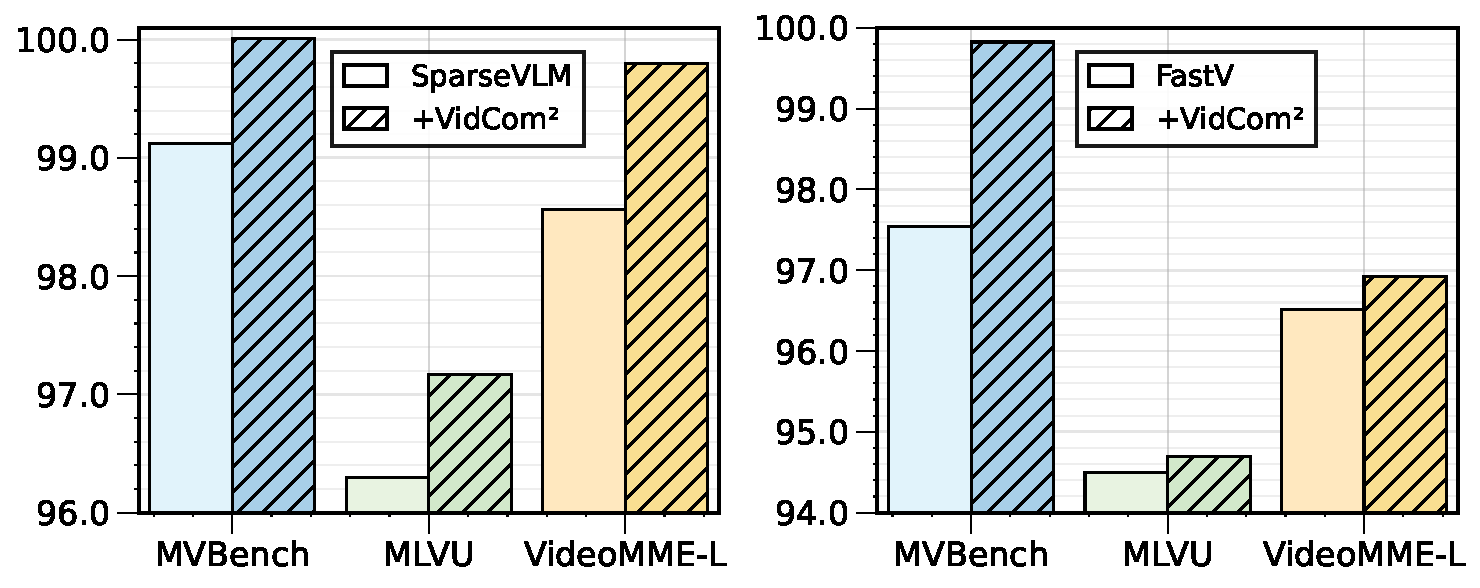
\includegraphics[width=\linewidth]{latex/figures/ablation_1_others.pdf}
    \vspace{-7mm}
    \caption{\textbf{Effects of Frame Compression Adjustment on other methods.}``+VidCom$^2$'' indicates the application of our Frame Compression Adjustment strategy.} 
    \vspace{-5mm}
\label{fig:ablation_1_others}
\end{figure}



% \noindent \textbf{Broader Applicability of VidCom$^2$.} 
\paragraph{Broad Applicability of Frame Compression Adjustment.}

Figure~\ref{fig:ablation_1_others} further demonstrates the effectiveness of integrating our Frame Compression Adjustment strategy with other methods. 

Results show consistent performance improvements compared to their original performance on LLaVA-OV-7B across short (MVBench) and long (MVLU and VideoMME-L) video understanding tasks. Notably, SparseVLM and FastV show significant gains on MVBench, where spatiotemporal changes are more pronounced. This improvement stems from the complementary nature of our approach: while Intra-LLM methods focus on \textbf{textual relevance}, our strategy considers \textbf{visual uniqueness}. This combination enables more comprehensive token preservation, capturing both distinctive visual content and instruction-relevant information, thus mitigating unique visual information loss that often occurs in text-centric approaches during token compression in LLM.





